\newpage
\section{Detaillierte Projektbeschreibung}
\begin{itemize}
    \item Umriss des Projekts, ohne zu sehr auf Details wie Regler, Potis, exakte Display-Technologie usw. einzugehen. Dazu da, um dem Leser eine Idee zu geben, worum es geht und wie wir uns die Funktionalität vorgestellt haben.
    \item Bild von Faceplate
    \item Audiosampler für Eurorack Modularsystem (was ist das?)
    \item Problem: Schwierig die "richtigen" Samples zu finden $\Rightarrow$ Klassifizierung der Samples
    \item Suchfilter über Hardware-Interface (Regler)
    \item Anzeige der passenden Samples auf dem Display
    \item Auswählen/Abspielen mit Poti
    \item Eurorack Standard
\end{itemize}

	\subsection{Modulare Synthesizer}
	
	In der modernen elektronischen Musikproduktion erfreut sich die Modularität von Synthesizern wieder großer Beliebtheit. 
	Die Methoden, verschiedene Module von unterschiedlichen Herstellern miteinander zu kombinieren, erleben ein Revival. 
	Wo einst die Reise der elektronischen Musik begann, werden diese Ansätze erneut aufgegriffen.
	
	In den 1950er Jahren erzeugten die Pioniere der elektronischen Musik mit Labor- und Testequipment neue Klänge. 
	Signalgeneratoren, Filter und anderes technisches Gerät aus den Ingenieurlabors wurden funktional zu Musikinstrumenten umgewandelt – die elektronische Musik war geboren.
	
	In den 1990er Jahren, durch die bessere Zugänglichkeit und günstigeren Kosten von Chips und Halbleitern, fand dieses Mindset den Weg zu den Consumer-Musikproduzenten - Dieter Doepfer entwickelte den Eurorack-Standard für modulare Synthesizer. 
	Es werden 3,5 mm Stecker und Buchsen verwendet, um die verschiedenen Module miteinander zu "verpatchen". 
	Dabei werden ausschließlich Monokabel und Monosignale genutzt. Über diese Steckverbindungen werden alle Nutzsignale, die für die Produktion der Töne mit dem Synthesizer erforderlich sind, übertragen. 
	Audiosignale, Steuersignale und Triggersignale werden mit denselben Buchsen verbunden.
	
	Dies eröffnet enorme Möglichkeiten, die Klangpalette zu erweitern. So können beispielsweise Audiosignale zur Steuerung der Parameter eines Moduls verwendet werden, was kreative und innovative Patches ermöglicht.
	
	Auch technisch haben sich modulare Synthesizer weiterentwickelt. 
	Es wird vermehrt auf digitale Module gesetzt. 
	Die Zeit der Analog-Puristen ist vorbei; alle Möglichkeiten der digitalen Signalverarbeitung werden genutzt, um innovative Module zu entwerfen, die neue Methoden und Ideen in das eigene Rack bringen.
	
	Eine Unterkategorie der digitalen Module bilden die Audiosampler. Diese Module nehmen digitale Aufnahmen (Samples) von Klängen oder Musikstücken auf, speichern und spielen sie ab. Die Samples können durch verschiedene Trigger aktiviert und in unterschiedlichen Tonhöhen und Geschwindigkeiten abgespielt werden. 
	Audiosampler ermöglichen es Musikern, realistische Klänge von Instrumenten, Stimmen oder Umweltgeräuschen in ihre Musik zu integrieren und kreativ zu manipulieren.
	
	\newpage
	\subsection{Das Konzept}
	
	Es gibt durchaus Audiosampler mit ergonomischer Steuerung, großen hochauflösenden Displays und zahlreichen Knöpfen, um diese komplexen Audiomaschinen angenehm zu steuern. 
	Beispiele hierfür sind die legendäre MPC von AKAI oder der Octatrack von Elektron. 
	Diese Geräte sind jedoch aufgrund ihrer Bedienelemente und der damit einhergehenden Ergonomie so groß, dass sie unmöglich in ein Eurorack unterzubringen sind und oft unzählige Untermenüs besitzen.
	
	\begin{wrapfigure}{r}{0.4\textwidth} % Increase the width of the figure environment
		\vspace{-20pt + 0.02\textwidth}
		\hspace{0.02\textwidth} % Add horizontal space
		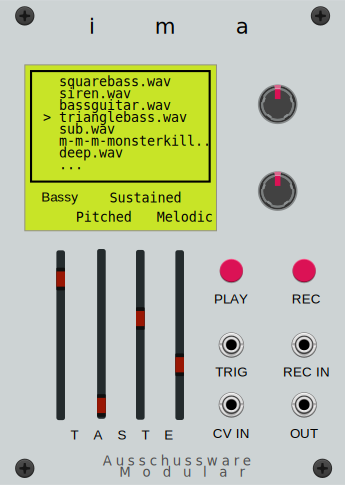
\includegraphics[width=0.38\textwidth]{pic/ima_mockup.png} % Keep the image size the same
		\caption{I M A Mockup Design}
		\vspace{-20pt}
	\end{wrapfigure}

	Daher sind Samplermodule im Eurorack-Standard häufig mit wenigen Features ausgestattet oder haben eine komplizierte, verschachtelte Bedienung. ``I M A`` (Intelligent Magic Audio) macht es Musikern hier deutlich einfacher! Der Schlüsselpunkt ist das gezielte Finden von Samples aus dem vorhandenen persistenten Speicher. Nur Samples des gewünschten Typs zu filtern, setzt normalerweise ein hohes Maß an manueller Sortierung und Ordnerstrukturierung voraus.
	
	
	Durch den neuronalgesteuerten Suchfilter von I M A kann eine Vorauswahl anhand musikalischer Parameter getroffen werden, ohne den kreativen Fluss des Künstlers zu unterbrechen.
	
	
	
	
